\documentclass[a4paper,12pt]{article}
\usepackage{amsmath}
\usepackage{pdfpages}
\usepackage[utf8]{inputenc}
\usepackage{hyperref}
\usepackage{listings}
\usepackage{xcolor}
 
\definecolor{codegreen}{rgb}{0,0.6,0}
\definecolor{codegray}{rgb}{0.5,0.5,0.5}
\definecolor{codepurple}{rgb}{0.0,0.58,0.82}
\definecolor{backcolour}{rgb}{0.95,0.95,0.92}

\lstdefinestyle{mystyle}{
    backgroundcolor=\color{backcolour},   
    commentstyle=\color{codegreen},
    keywordstyle=\color{magenta},
    numberstyle=\tiny\color{codegray},
    stringstyle=\color{codepurple},
    basicstyle=\ttfamily\footnotesize,
    breakatwhitespace=false,         
    breaklines=true,                 
    captionpos=b,                    
    keepspaces=true,                 
    numbers=left,                    
    numbersep=5pt,                  
    showspaces=false,                
    showstringspaces=false,
    showtabs=false,                  
    tabsize=2
}

\lstset{style=mystyle}

\title{Contol theory Homework \#1 report}
\author{Anton Brisilin, BS18-02 Student}
\date{\today}
\begin{document}
\maketitle
\section{Task 1.}
Given equation:
$$x''-5x=x'+t+2x+3, x'(0)=4, x(0)=3$$
Simplified DE:
$$x''=x'+7x+t+3$$
Simulink schema (w/o transfer function block):
\begin{center}
    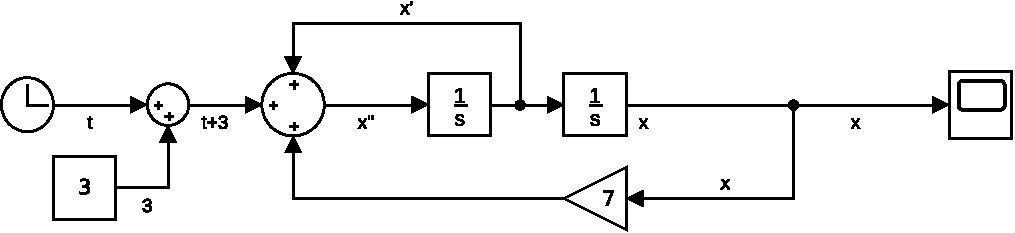
\includegraphics[width=\linewidth]{Schema1.pdf}
\end{center}
Calculation of transfer function:\\
Given equation:
$$x''=x'+7x+t+3, x'(0)=4, x(0)=3$$
Introduce new operator: $p=\frac{d}{dt}$
$$p^2x = px+7x+t+3$$
$$x(p^2-p-7)=t+3$$
$$x=\frac{1}{(p^2-p-7)}(t+3)$$
Therefore, our transfer function is 
$$T=\frac{1}{(s^2-s-7)}$$
Now we can build Simulink schema with transfer function 
block to solve our DE. Needs to note, that transfer 
function is designed for very simple cases, when initial 
conditions are all zero.\\
Simulink schema (with transfer function block):
\begin{center}
    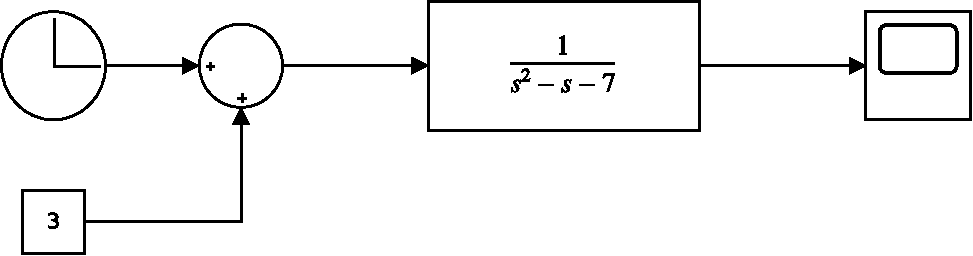
\includegraphics[width=\linewidth]{Schema2.pdf}
\end{center}
Matlab code with solution using Laplace Transform:
\begin{lstlisting}[language=matlab]
    syms t x(t) s X;
    % Given equation
    dx = diff(x,t);
    d2x = diff(x,t,2);
    equation = d2x == dx + 7*x + t + 3;
    % Laplace transform
    trans = laplace(equation,t,s);
    % Substituting initial conditions
    trans = subs(trans, [laplace(x,t,s), dx(0), x(0)], [X,4,3]);
    % Solving for X
    sol = solve(trans,X);
    % Inverse Laplace transform
    sol =  ilaplace(sol, s, t);
    % Plotting the solution
    fplot(sol, [0 10])
\end{lstlisting}
Matlab code with solution of an equation with dsolve:
\begin{lstlisting}[language=matlab]
    syms x(t);
    equation = diff(x,t,2) == diff(x,t) + 7*x + t + 3;
    % Adding conditions for given IVP
    cond1 = x(0) == 3;
    Dx=diff(x,t);
    cond2 = Dx(0) == 4;
    cond = [cond1,cond2];
    % Using dsolve to obtain exact symbolic solution
    sol = dsolve(eqn,cond);
    % Plotting solution
    fplot(sol,[0 10]);
\end{lstlisting} 
\subsection{Plot of the solution}
\begin{center}
    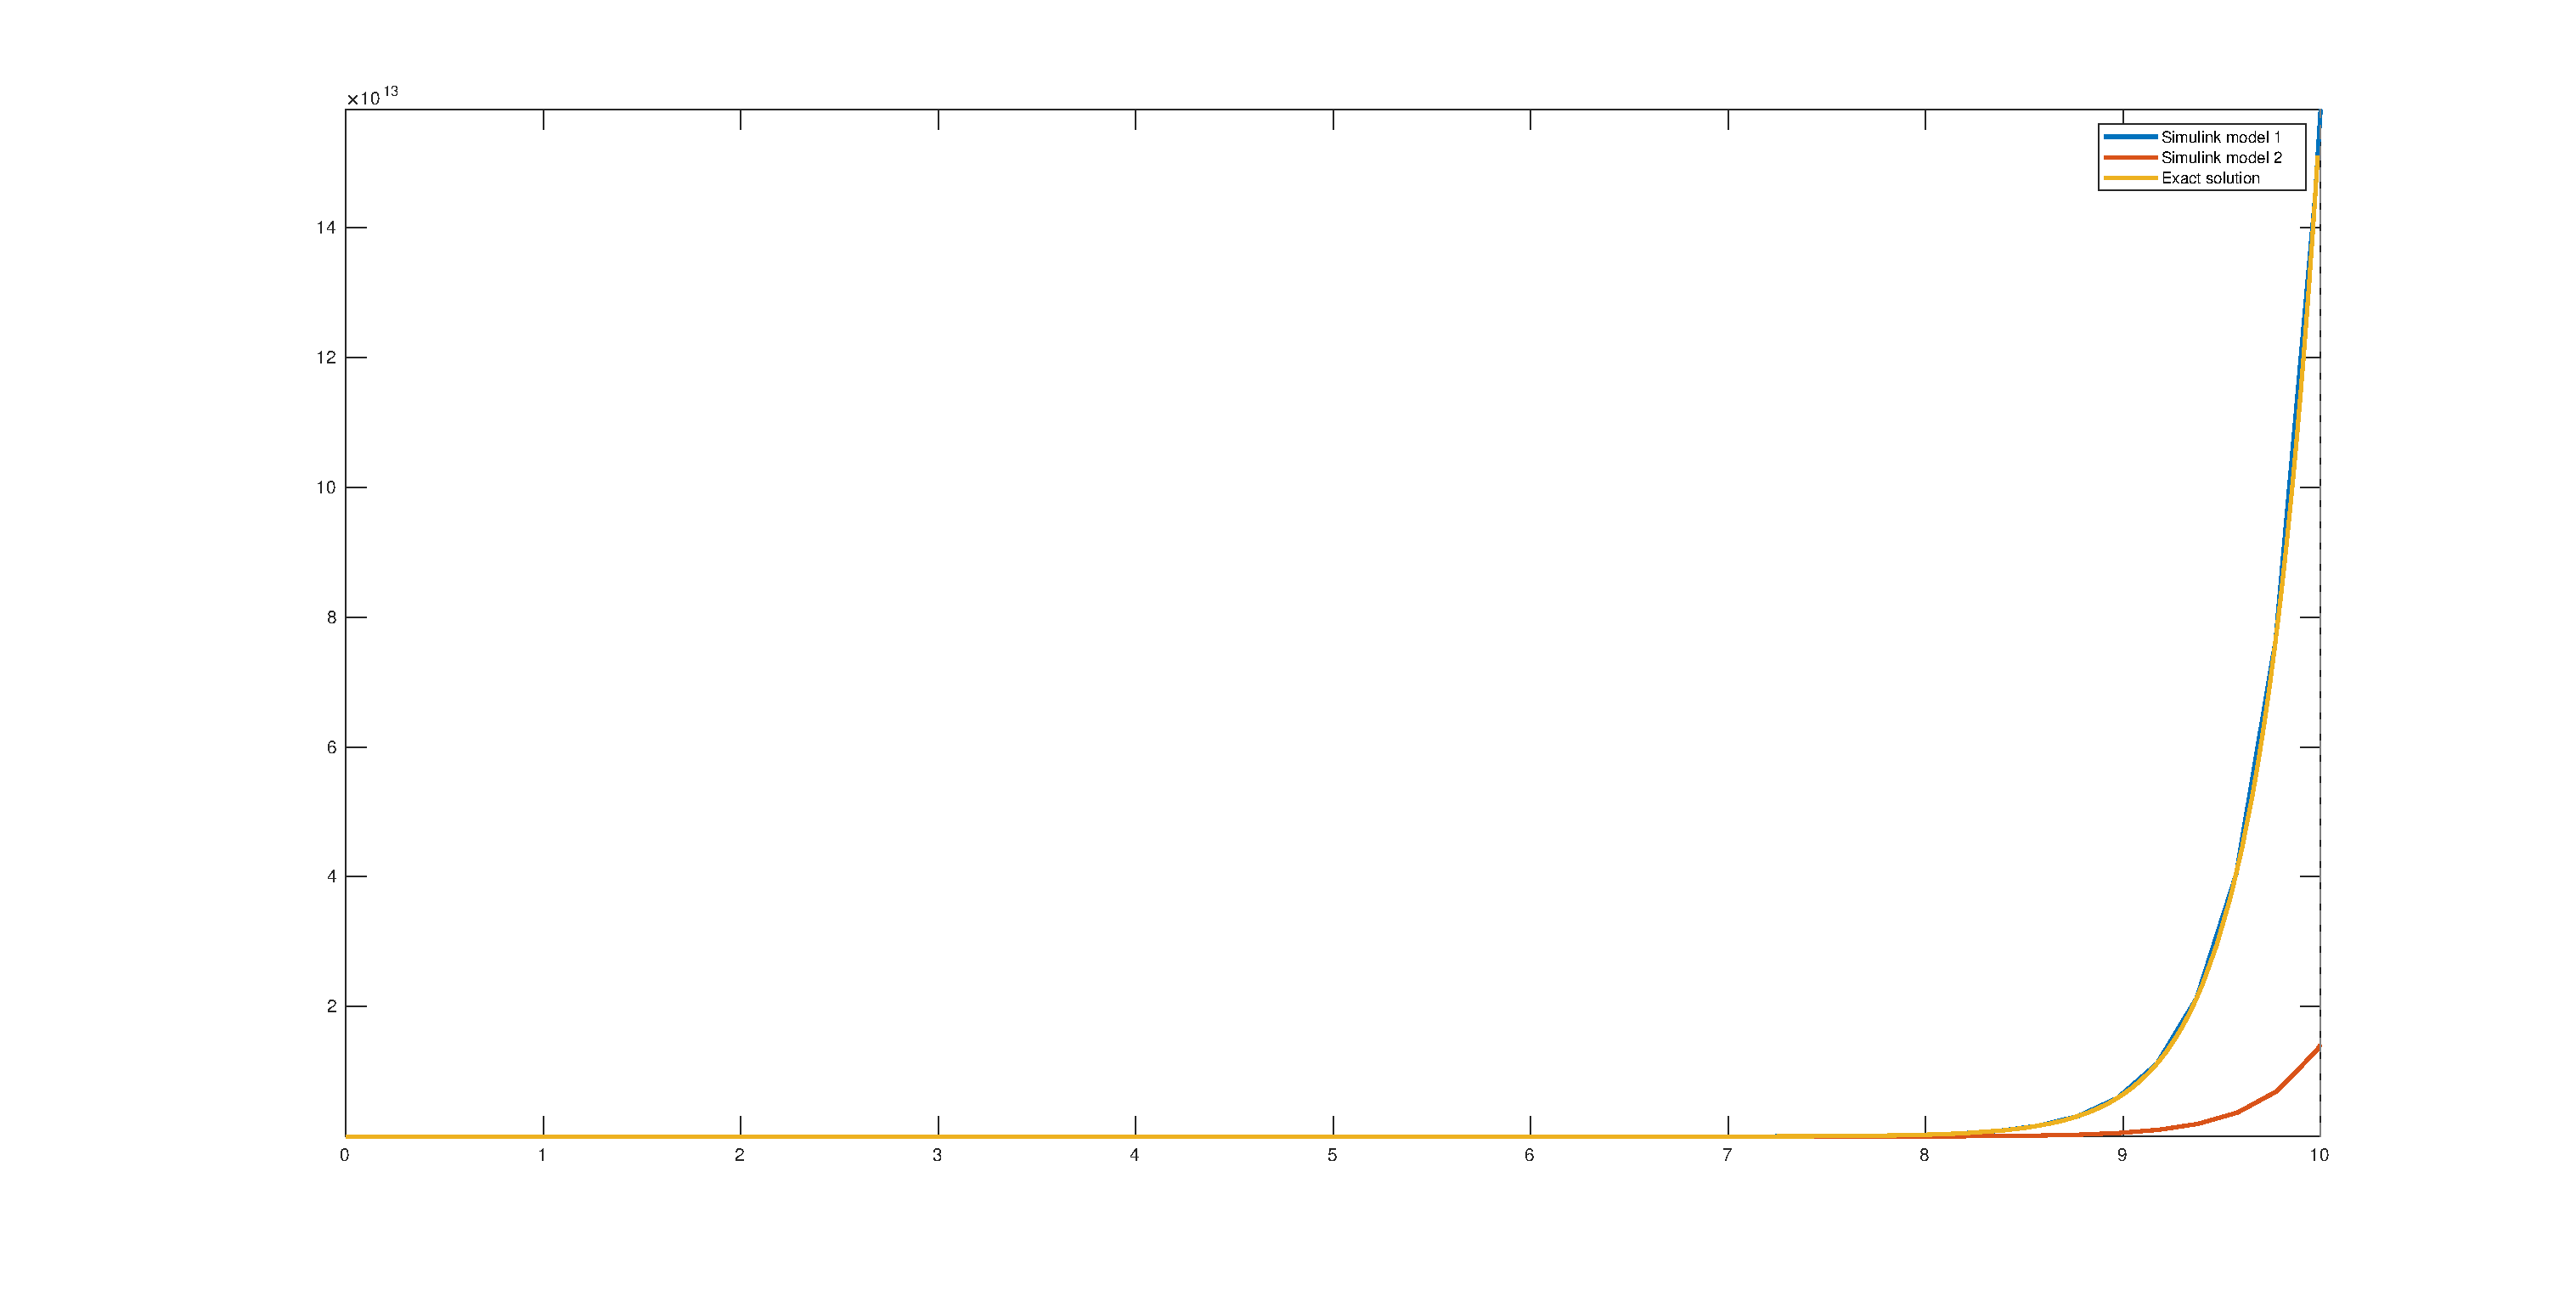
\includegraphics[width=\linewidth]{totalPlot.eps}
    Plots of solutions obtained with different methods. 
    Solution with symbolic Laplace transform was omited, 
    because it differs from solution obtained by dsolve()
    less than by $10^{-12}$
\end{center}

\section{Task 2.}
Given system:
$$3x'''+3x'-3=2t-2, y=3x'$$
After simplification:
$$x''=-x'+\frac{2}{3}t+\frac{1}{3}$$
$$\begin{cases}
    x=x_1\\
    x_1'=x_2\\
    x_2'=-x_2+\frac{2}{3}t+\frac{1}{3}
\end{cases}$$
Hence, state-space representation of our system is:
\begin{equation*}
    \begin{bmatrix}
        x_1'\\x_2'
    \end{bmatrix}
    =
    \begin{bmatrix}
        0 & 1\\
        0 & -1
    \end{bmatrix}
    \cdot
    \begin{bmatrix}
        x_1 \\ x_2
    \end{bmatrix}
    +
    \begin{bmatrix}
        \frac{2}{3} & 0 \\
        0 & \frac{1}{3}
    \end{bmatrix}
    \begin{bmatrix}
        t \\ 1
    \end{bmatrix}
\end{equation*}
\begin{equation*}
    \begin{bmatrix}
        y
    \end{bmatrix}
    =
    \begin{bmatrix}
        0 & 1
    \end{bmatrix}
    \cdot
    \begin{bmatrix}
        x_1 \\ x_2
    \end{bmatrix}
    +
    \begin{bmatrix}
        0
    \end{bmatrix}
    \begin{bmatrix}
        t \\ 1
    \end{bmatrix}
\end{equation*}

\section{Task 3.}
Given system:
$$
\begin{cases}
    3\ddddot{x}+2\dddot{x}-3\ddot{x}+2\dot{x}-3=u_1+5u_2\\
    y=\dot{x}+u2
\end{cases}
$$
Convert to space-state:
$$
\begin{cases}
    x=x_1\\
    \dot{x_1}=x_2\\
    \dot{x_2}=x_3\\
    \dot{x_3}=x_4\\
    \dot{x_4}=-\frac{2}{3}x_4+x_3+-\frac{2}{3}x_2
    +\frac{5}{3}u_2+\frac{1}{3}u_2+1\\
    y=x_2+u_2
\end{cases}
$$
\begin{equation*}
    \begin{bmatrix}
        \dot{x_1}\\ \dot{x_2} \\
        \dot{x_3}\\ \dot{x_4}
    \end{bmatrix}
    =
    \begin{bmatrix}
        0 & 1 & 0 & 0\\
        0 & 0 & 1 & 0\\
        0 & 0 & 0 & 1\\
        0 & -\frac{2}{3} & 1 & -\frac{2}{3}
    \end{bmatrix}
    \cdot
    \begin{bmatrix}
        x_1 \\ x_2 \\ x_3 \\x_4
    \end{bmatrix}
    +
    \begin{bmatrix}
        0 & 0 & 0 \\
        0 & 0 & 0 \\
        0 & 0 & 0 \\
        1 & \frac{1}{3} & \frac{5}{3}
    \end{bmatrix}
    \begin{bmatrix}
        1 \\ u_1 \\ u_2
    \end{bmatrix}
\end{equation*}
\begin{equation*}
    \begin{bmatrix}
        y
    \end{bmatrix}
    =
    \begin{bmatrix}
        0 & 1 & 0 & 0
    \end{bmatrix}
    \cdot
    \begin{bmatrix}
        x_1 \\ x_2 \\ x_3 \\ x_4
    \end{bmatrix}
    +
    \begin{bmatrix}
        0 & 0 & 1
    \end{bmatrix}
    \begin{bmatrix}
        1 \\ u_1 \\ u_2
    \end{bmatrix}
\end{equation*}
\end{document}